\chapter{Động lực học Friedmann và phương trình trạng thái}

\lectureoverview{Sự giãn nở đồng nhất phải được tách biệt khỏi vật lý của các hệ liên kết cục bộ, và hình học nội tại phải được tách biệt khỏi hình dạng của một phép nhúng. Khi những phân biệt đó đã được xác lập, nguyên lý vũ trụ học rút metric không-thời gian về một thừa số tỉ lệ \(a(t)\) và một nhãn độ cong \(k\). Khi đó, thành phần thời gian-thời gian của phương trình Einstein trở thành phương trình năng lượng Friedmann. Để giải nó, ta vẫn cần quan hệ của môi chất liên hệ áp suất với mật độ năng lượng. Nhiệt động lực học đoạn nhiệt và phương trình trạng thái \(P=w\rho\) cho \(\rho\propto a^{-3(1+w)}\), hợp nhất vật chất, bức xạ và năng lượng chân không trong một khuôn khổ.}

\section{Những câu hỏi định hình bức tranh vật lý}

\subsection{Không gian có thể lặp lại trước chân trời không?}

Một vũ trụ phẳng hữu hạn có thể được biểu diễn bằng một ô tuần hoàn. Nếu ô đó nhỏ hơn vùng quan sát được, ánh sáng có thể đi xuyên qua nó và bầu trời sẽ chứa các hình ảnh lặp lại của cùng những cấu trúc ấy. Việc phát hiện các sự lặp lại đó khó hơn nhiều so với chỉ đơn giản nhận ra một thiên hà quen thuộc: các ảnh đến từ những hướng và những thời kỳ khác nhau, và bị biến đổi bởi tiến hóa vũ trụ. Tuy vậy, tô pô tuần hoàn có những hệ quả quan sát được.

\begin{classroomqa}
\audiencequestion{Liệu toàn bộ vũ trụ có thể nhỏ hơn vùng quan sát được không?}
\lecturerresponse{Một xuyến được đồng nhất tuần hoàn là đề xuất tự nhiên. Khi đó, chúng ta sẽ quan sát các bản sao lặp lại của cùng một vùng vật lý, theo nghĩa hình tượng là nhìn thấy chính mình qua cửa sau. Các cuộc tìm kiếm tính tuần hoàn vũ trụ tương ứng đã không tạo ra bằng chứng ủng hộ, và quả thật có đặt ra các ràng buộc đối với những ô cơ bản nhỏ. Khả năng này là nhất quán về mặt hình học, nhưng bằng chứng này không ủng hộ một vũ trụ nhỏ hơn vùng đã được quan sát. \lecturetimestamp{00:01:17--00:02:33}}
\end{classroomqa}

\subsection{Sự giãn nở không kéo tách các hệ liên kết}

Sự giãn nở vũ trụ mô tả chuyển động trên quy mô lớn của vật chất chuyển động tự do trong hình học vũ trụ học trung bình. Nó không phải là một mệnh lệnh phổ quát buộc mọi độ dài riêng đều phải tăng. Lực điện từ liên kết các nguyên tử, hấp dẫn liên kết các hệ hành tinh, và các lực phân tử thông thường liên kết các vật rắn. Các tương tác này mạnh hơn rất nhiều so với hiệu chỉnh vũ trụ học ở những thang đó.

\begin{classroomqa}
\audiencequestion{Sự giãn nở có phải do năng lượng tối gây ra không, và vì sao các nguyên tử hoặc quỹ đạo hành tinh không giãn nở cùng với không gian?}
\lecturerresponse{Vũ trụ đã được biết là đang giãn nở trước khi năng lượng tối được phát hiện. Năng lượng tối làm thay đổi sự giãn nở bằng cách gia tốc nó; nó không phải là định nghĩa hay nguyên nhân ban đầu của sự giãn nở. Một hệ liên kết không đi theo dòng Hubble vì các lực cục bộ của nó chi phối. Một nền đang gia tốc có thể tạo ra một nhiễu loạn cực kỳ nhỏ đối với một nguyên tử hay một quỹ đạo, nhưng liên kết thông thường khôi phục một trạng thái cân bằng gần như không đổi thay vì cho phép hệ bay tách ra. \lecturetimestamp{00:02:36--00:06:50}}
\end{classroomqa}

\subsection{Năng lượng trong một hình học phụ thuộc thời gian}

Phản đối còn lại không liên quan đến lực mà liên quan đến việc hạch toán. Nếu một quỹ đạo liên kết liên tục chống lại một nhiễu loạn vũ trụ học nhỏ, năng lượng cần thiết đến từ đâu? Tiền đề này mang một định luật bảo toàn từ một nền tĩnh vào một không-thời gian không có đối xứng tịnh tiến theo thời gian toàn cục.

\begin{classroomqa}
\audiencequestion{Năng lượng đến từ đâu khi liên kết cục bộ chống lại sự giãn nở?}
\lecturerresponse{Bảo toàn năng lượng trong một thế giới tĩnh suy ra từ bất biến tịnh tiến theo thời gian: nền và các định luật của nó trông như nhau khi một thí nghiệm bị tịnh tiến theo thời gian. Một không-thời gian đang giãn nở không bất biến đối với tịnh tiến theo thời gian theo nghĩa toàn cục đó, nên không nhất thiết phải có một tổng năng lượng bảo toàn duy nhất cho toàn thể vũ trụ. Bảo toàn năng lượng-xung lượng cục bộ vẫn đúng và sẽ xuất hiện bên dưới dưới dạng phương trình liên tục. Điều không còn đúng là khẳng định ngây thơ rằng một năng lượng vũ trụ được xác định toàn cục phải giữ nguyên trong khi hình học thay đổi. \lecturetimestamp{00:06:52--00:09:24}}
\end{classroomqa}

\subsection{Tính đồng nhất là một phát biểu ở mức mô tả thô}

Nguyên lý vũ trụ học phụ thuộc vào thang đo. Không khí trong một căn phòng kín có thể gần như đồng đều ở thang của căn phòng nhưng có tính hạt ở thang phân tử. Vũ trụ tương tự cũng chứa các hành tinh, thiên hà, các cụm và các thăng giáng mật độ. Tính đồng nhất và đẳng hướng nói đến hành vi trung bình của nó trên những khoảng cách đủ lớn để các cấu trúc ấy không còn chọn ra một vị trí hay một hướng nào nữa.

\begin{classroomqa}
\audiencequestion{Các cấu trúc liên kết ở thang nhỏ có mâu thuẫn với tính đồng nhất và đẳng hướng không?}
\lecturerresponse{Không. Tính đồng nhất chính xác không đúng ở thang nhỏ, cũng như nó không đúng đối với không khí khi ta phân giải được từng phân tử riêng lẻ. Ở các thang cỡ hàng trăm triệu năm ánh sáng trở lên, phân bố quan sát được là xấp xỉ đồng đều và không phụ thuộc hướng. Bên ngoài vùng ta có thể quan sát, tính đồng nhất vẫn là một giả định mà các hệ quả của nó phải được kiểm nghiệm chứ không phải một sự kiện đã được xác lập. \lecturetimestamp{00:09:27--00:10:55}}
\end{classroomqa}

\section{Tính đồng nhất và đẳng hướng như các phát biểu về metric}

Tính đồng nhất và đẳng hướng là những phát biểu hình học trước khi chúng trở thành những phát biểu động lực học. Phương trình Einstein sẽ cho ta biết hình học thay đổi theo thời gian như thế nào. Trước hết ta phải nói rõ loại hình học không gian nào được phép tại mỗi thời điểm.

\begin{classroomqa}
\audiencequestion{Về mặt toán học, tính đồng nhất và đẳng hướng có nghĩa là gì?}
\lecturerresponse{Mô tả không gian bằng một metric và chọn các tọa độ \(x^i\) lấy một điểm làm gốc. Bây giờ chọn các tọa độ \(y^i\) lấy một điểm khác làm gốc. Tính đồng nhất có nghĩa là tồn tại một phép biến đổi có thể dời gốc tọa độ mà vẫn để metric có cùng dạng hàm. Khi đó mọi điểm đều tương đương về mặt hình học với mọi điểm khác. Tính đẳng hướng bổ sung đối xứng quay quanh mỗi điểm, nên không có hướng nào được ưu tiên. \lecturetimestamp{00:11:13--00:14:26}}
\end{classroomqa}

\begin{definition}
Một không gian là \emph{đồng nhất} nếu một phép đẳng cự có thể đưa bất kỳ điểm nào tới bất kỳ điểm nào khác. Nó là \emph{đẳng hướng} quanh một điểm nếu các phép quay quanh điểm đó không làm thay đổi hình học của nó. Một không gian vừa đồng nhất vừa đẳng hướng thì không có vị trí ưu tiên cũng không có hướng ưu tiên.
\end{definition}

Mặt phẳng Euclid làm cho định nghĩa trở nên minh bạch. Trong tọa độ Descartes,
\begin{equation}
ds^2=dx_1^2+dx_2^2.
\label{eq:c04-flat-metric}
\end{equation}
Dời gốc tọa độ đi các hằng số \(a_1\) và \(a_2\):
\begin{equation}
y_1=x_1+a_1,
\qquad
y_2=x_2+a_2.
\label{eq:c04-flat-translation}
\end{equation}
Vì \(dy_i=dx_i\), metric sau phép tịnh tiến là
\begin{equation}
ds^2=dy_1^2+dy_2^2.
\end{equation}
Các ký hiệu dùng để gán nhãn điểm đã thay đổi, nhưng quy tắc khoảng cách thì không. Đây là cách hiện thực hóa đơn giản nhất của tính đồng nhất. Các phép quay cũng bảo toàn metric, nên mặt phẳng cũng đẳng hướng.

Mặt cầu kém tầm thường hơn chỉ vì tọa độ của nó kém thuận tiện hơn. Chọn cực nam làm gốc, mặt hai-cầu đơn vị có thể viết là
\begin{equation}
d\Omega_2^2=dr^2+\sin^2 r\,d\theta^2.
\label{eq:c04-sphere-metric}
\end{equation}
Xoay mặt cầu sao cho một cực đông trở thành gốc mới. Phép biến đổi tọa độ thì rườm rà, nhưng kết quả lại vẫn là phương trình~\eqref{eq:c04-sphere-metric}. Không có điểm nào trên một mặt cầu tròn được phân biệt về mặt hình học.

\begin{classroomqa}
\audiencequestion{Một xuyến phẳng được đồng nhất tuần hoàn có vừa đồng nhất vừa đẳng hướng không?}
\lecturerresponse{Nó đồng nhất dưới các phép tịnh tiến: mọi điểm trong ô tuần hoàn đều có cùng hình học cục bộ. Nó không hoàn toàn đẳng hướng, vì các phép đồng nhất chọn ra những hướng và độ dài tuần hoàn ưu tiên. Nhìn dọc theo một trong các trục ấy khác về mặt toàn cục so với nhìn theo một hướng xiên bất kỳ. Vì thế xuyến cung cấp một ví dụ rõ ràng về tính đồng nhất mà không có đẳng hướng hoàn toàn. \lecturetimestamp{00:20:18--00:21:30}}
\end{classroomqa}

Sự đồng đều quan sát được ở quy mô lớn là động lực cho nguyên lý vũ trụ học trong phạm vi chân trời của chúng ta. Việc mở rộng nó ra ngoài vùng quan sát được là một tiên đề, không phải một quan sát trực tiếp. Chúng ta chấp nhận tiên đề đó vì nó cho một hình học được xác định rõ ràng, mà các hệ quả của nó có thể được đối chiếu với dữ liệu.

\section{Hình học nội tại và phép nhúng}

Khi nói không gian là hình cầu, ta dễ hình dung bề mặt cao su của một quả bóng bay đặt trong một căn phòng lớn hơn. Hình ảnh đó có thể giúp ta vẽ, nhưng căn phòng xung quanh không phải là một phần của khẳng định vũ trụ học. Hình học quan trọng là \emph{nội tại}: nó gồm các khoảng cách và góc mà những quan sát viên vẫn ở trong không gian có thể đo được.

\subsection{Các thế giới một chiều khép kín}

Hãy xét một thế giới một chiều khép kín. Ta có thể vẽ nó thành một đường tròn, một hình vuông với các góc bo tròn, hoặc một vòng hình đậu phộng. Một cư dân bị giới hạn trên đường đó chỉ đo khoảng cách dọc theo nó. Nếu hai vòng có cùng tổng chu vi, thì những cư dân ấy gặp cùng một hình học nội tại ngay cả khi các hình vẽ trông hoàn toàn khác nhau.

\begin{figure}[htbp]
\centering
\includegraphics[width=0.72\textwidth]{lecture_04_figure_05.png}
\caption{Các vòng khép kín tròn và biến dạng được dùng để phân biệt hình học nội tại với hình dạng của phép nhúng. Khung hình ở thời điểm muộn hơn này giữ lại các hình vẽ đã được thực hiện trong phần thảo luận trước đó; nội dung liên quan xuất hiện tại 00:23:21--00:25:59.}
\label{fig:c04-intrinsic-board}
\lectureframe{00:59:54.899}
\end{figure}

Mọi metric một chiều đều phẳng cục bộ. Một đoạn dây ngắn có thể được duỗi thẳng mà không cần kéo dãn, nên sự uốn cong nhìn thấy được trong mặt phẳng xung quanh là độ cong ngoại tại chứ không phải độ cong nội tại. Một vòng kín có một môđun toàn cục, tức là chu vi của nó, nhưng không có sự uốn cong cục bộ nội tại nào mà các cư dân một chiều của nó có thể đo được.

\begin{figure}[htbp]
\centering
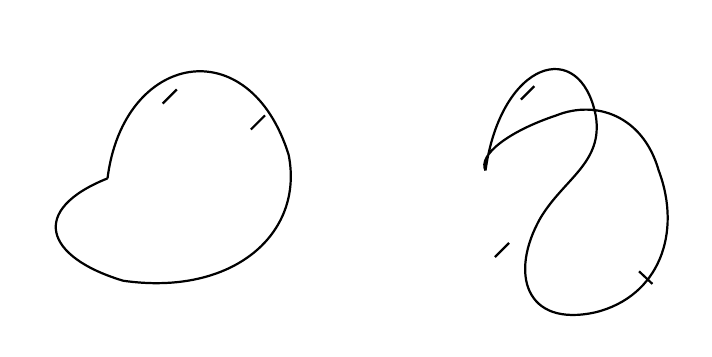
\begin{tikzpicture}[scale=1.0]
\draw[line width=0.8pt] (0,0)
  .. controls (0.2,1.6) and (1.8,1.9) .. (2.3,0.3)
  .. controls (2.5,-0.7) and (1.6,-1.5) .. (0.2,-1.3)
  .. controls (-0.8,-1.0) and (-1.0,-0.4) .. (0,0);
\draw[line width=0.8pt] (0.70,0.95) -- (0.88,1.13);
\draw[line width=0.8pt] (1.82,0.62) -- (2.00,0.80);

\draw[line width=0.8pt] (4.8,0.1)
  .. controls (5.0,1.5) and (6.0,1.8) .. (6.2,0.8)
  .. controls (6.3,0.2) and (5.8,0.0) .. (5.5,-0.5)
  .. controls (5.1,-1.2) and (5.3,-1.9) .. (6.2,-1.7)
  .. controls (7.0,-1.5) and (7.3,-0.7) .. (7.0,0.1)
  .. controls (6.8,0.8) and (6.2,1.0) .. (5.7,0.8)
  .. controls (5.1,0.6) and (4.7,0.3) .. (4.8,0.1);
\draw[line width=0.8pt] (5.25,1.00) -- (5.42,1.17);
\draw[line width=0.8pt] (5.10,-0.82) -- (4.92,-1.00);
\draw[line width=0.8pt] (6.75,-1.18) -- (6.92,-1.34);
\end{tikzpicture}
\caption{Bản dựng lại rõ ràng của đường tròn và vòng kín bị biến dạng. Chu vi bằng nhau có nghĩa là hình học nội tại một chiều như nhau.}
\label{fig:c04-intrinsic-redraw}
\end{figure}

\begin{classroomqa}
\audiencequestion{Một đoạn thẳng hữu hạn có phải là cùng một loại không gian một chiều không?}
\lecturerresponse{Không. Một đoạn thẳng có hai đầu mút, còn một vòng kín thì không có. Sự phân biệt tôpô đó là nội tại và không thể bị loại bỏ bằng cách uốn một trong hai đối tượng trong một không gian lớn hơn. Khi tôpô đã cố định, cái trước được đặc trưng bởi độ dài, còn cái sau bởi chu vi. \lecturetimestamp{00:26:00--00:26:39}}
\end{classroomqa}

\subsection{Vì sao các phép nhúng hữu ích nhưng không bắt buộc}

Ta hình dung một đường tròn một chiều bằng cách đặt nó trong hai chiều và một mặt cầu hai chiều bằng cách đặt nó trong ba chiều. Mô thức ấy khiến ta muốn đòi hỏi một chiều Euclid thứ tư trước khi bàn về 3-cầu. Đòi hỏi đó phản ánh trực quan của con người, không phải một tất yếu toán học. Hệ thống thị giác của chúng ta đã tiến hóa để định hướng trong ba chiều; tọa độ và metric cho phép ta suy luận vượt quá giới hạn đó mà không cần dựng nên một điểm nhìn bên ngoài theo nghĩa đen.

\begin{classroomqa}
\audiencequestion{Liệu có thể tồn tại các chiều không gian bổ sung nhưng quá nhỏ để nhìn thấy không?}
\lecturerresponse{Có. Hình học không đòi hỏi mọi chiều phải có cùng độ lớn quan sát được. Một chiều compact có thể nhỏ hơn rất nhiều so với các thang mà kinh nghiệm thông thường thăm dò. Tuy nhiên, điểm cốt yếu ở đây còn đơn giản hơn: dù các chiều phụ có tồn tại về mặt vật lý hay không, vẫn không cần đến một chiều nhúng để định nghĩa metric nội tại của không gian ba chiều của chúng ta. \lecturetimestamp{00:29:55--00:30:12}}
\end{classroomqa}

\begin{classroomqa}
\audiencequestion{Làm sao một cư dân bị giới hạn trên một đường cong biết được đường đó có bị uốn không?}
\lecturerresponse{Người đó không thể biết chỉ từ các phép đo nội tại. Hãy hình dung ánh sáng và vật chất bị giam trong một sợi quang. Uốn sợi đó mà không kéo dãn làm thay đổi phép nhúng, nhưng không làm thay đổi các khoảng cách hay thời gian truyền tín hiệu đo dọc theo sợi. Chỉ một tín hiệu thoát ra không gian xung quanh mới có thể cho biết sự uốn cong bên ngoài. \lecturetimestamp{00:30:15--00:31:14}}
\end{classroomqa}

Thí nghiệm tưởng tượng này có thể được cụ thể hóa thành một phép kiểm tra. Một sinh vật bị giới hạn trong sợi có thể phát đi một tín hiệu, chẳng hạn một photon đủ năng lượng, và chỉ có thể phát hiện ra một hướng bên ngoài nếu tín hiệu thoát khỏi sợi rồi về sau quay trở lại theo một lộ trình không tồn tại trong metric một chiều. Theo đúng tinh thần đó, mệnh đề rằng không gian thông thường có ba chiều lớn rốt cuộc là một kết luận thực nghiệm, chứ không phải một suy diễn từ những gì tâm trí con người có thể hình dung.

\begin{classroomqa}
\audiencequestion{Nếu mọi không gian một chiều đều phẳng cục bộ, thì mọi không gian hai chiều cũng phải phẳng cục bộ hay không?}
\lecturerresponse{Không. Một tấm được cuộn thành hình trụ vẫn phẳng về mặt nội tại: nó có thể được trải ra mà không cần kéo dãn. Một bán cầu không thể được làm phẳng lên một mặt phẳng mà không kéo dãn hoặc xé rách, nên nó có độ cong nội tại. Mọi mảnh đủ nhỏ đều trông xấp xỉ Euclid, nhưng các độ lệch đo được xuất hiện ở thang hữu hạn. Sự tương phản giữa hình trụ và hình cầu chính là sự tương phản giữa sự uốn cong ngoại tại và độ cong nội tại. \lecturetimestamp{00:31:14--00:35:00}}
\end{classroomqa}

\begin{classroomqa}
\audiencequestion{Độ cong nội tại có nhất thiết nghĩa là có mặt một trường hấp dẫn không?}
\lecturerresponse{Trong thuyết tương đối rộng, độ cong không-thời gian là biểu hiện bất biến của hấp dẫn thủy triều. Vì thế độ cong không gian vũ trụ \(k/a^2\) là một phần của hình học hấp dẫn, chứ không chỉ đơn thuần là một sự uốn cong trong một không gian bên ngoài được tưởng tượng ra. Vật chất ảnh hưởng đến độ cong thông qua phương trình Einstein, nhưng không nên đẩy phát biểu ấy tới mức thành "độ cong chỉ tồn tại ở nơi có vật chất": không-thời gian chân không có thể mang độ cong Weyl, như ở bên ngoài một ngôi sao hoặc trong một sóng hấp dẫn. \lecturetimestamp{00:35:01--00:35:51}}
\end{classroomqa}

Bây giờ ta áp đặt phép lý tưởng hóa ở quy mô lớn. Lấy trung bình trên các sao, các thiên hà, các cụm thiên hà và những bất quy tắc cục bộ, cũng như khi ta bỏ qua núi non để mô tả Trái Đất là tròn. Hình học không gian thu được được coi là đồng nhất và đẳng hướng. Dưới các giả thiết này có ba khả năng độ cong hằng: phẳng, cầu và hyperbolic.

\section{Ansatz FRW và ba trường hợp độ cong}

Các giả thiết đối xứng rút hình học xuống còn một hệ số tỉ lệ phụ thuộc thời gian và một dấu độ cong rời rạc. Trong tọa độ đồng chuyển động, ansatz Friedmann-Robertson-Walker là
\begin{equation}
ds^2=-dt^2+a(t)^2\,d\Sigma_k^2,
\qquad
k\in\{-1,0,+1\}.
\label{eq:c04-frw}
\end{equation}
Tọa độ thời gian là thời gian riêng của các quan sát viên đồng chuyển động. Tính đồng nhất cho phép \(a\) phụ thuộc vào thời gian nhưng không phụ thuộc vào vị trí, còn tính đẳng hướng cấm một hướng không gian ưu tiên.

\begin{figure}[htbp]
\centering
\includegraphics[width=0.74\textwidth]{lecture_04_figure_02.png}
\caption{Ba metric không gian độ cong hằng được nhóm dưới cùng một thừa số tỉ lệ chung. Khung hình này được chụp về sau, sau khi trên bảng đã có thêm những nội dung khác, nhưng nó vẫn giữ lại phần thảo luận về metric từ 00:40:23--00:42:42.}
\label{fig:c04-frw-board}
\lectureframe{00:45:48.386}
\end{figure}

Dùng tọa độ xuyên tâm \(r\) và metric 2-cầu đơn vị \(d\Omega_2^2\), ba metric không gian chuẩn hóa là
\begin{align}
d\Sigma_0^2 &= dr^2+r^2d\Omega_2^2,
&& k=0,
\label{eq:c04-flat-space}\\
d\Sigma_{+1}^2 &= dr^2+\sin^2 r\,d\Omega_2^2,
&& k=+1,
\label{eq:c04-spherical-space}\\
d\Sigma_{-1}^2 &= dr^2+\sinh^2 r\,d\Omega_2^2,
&& k=-1.
\label{eq:c04-hyperbolic-space}
\end{align}
Vì thế, tại một thời điểm cố định, không gian là phẳng, cong dương hoặc cong âm. Nhân với \(a(t)^2\) làm thay đổi mọi khoảng cách không gian theo cùng một hệ số, đồng thời bảo toàn hình dạng đã chuẩn hóa.

Xét hai thiên hà có độ tách đồng chuyển động cố định \(\Delta\chi\). Khoảng cách vật lý của chúng là
\begin{equation}
D(t)=a(t)\Delta\chi.
\end{equation}
Lấy đạo hàm và khử \(\Delta\chi\) thu được
\begin{equation}
\dot D=\dot a\,\Delta\chi
      =\frac{\dot a}{a}D
      =H(t)D,
\qquad
H(t)\equiv\frac{\dot a}{a}.
\label{eq:c04-hubble-law}
\end{equation}
Do đó định luật Hubble suy ra về mặt động học từ sự co giãn đồng nhất. Tham số Hubble có thể thay đổi theo thời gian, nhưng tại bất kỳ thời gian vũ trụ cố định nào nó cũng như nhau ở khắp mọi nơi.

\section{Từ phương trình Einstein đến phương trình Friedmann}

Metric cho biết các khoảng cách được đo như thế nào, nhưng không cho biết \(a(t)\) tiến hóa ra sao. Không-thời gian cong đòi hỏi phương trình Einstein. Việc tính mọi ký hiệu Christoffel và mọi thành phần độ cong sẽ làm mờ lập luận vật lý, vì vậy ta dùng dạng do đối xứng quy định và tách riêng thành phần thời gian-thời gian của nó.

Trong hệ đơn vị với \(c=1\) và tạm thời bỏ qua hằng số vũ trụ học, phương trình tensor đầy đủ là
\begin{equation}
G_{\mu\nu}
\equiv
R_{\mu\nu}-\frac12 g_{\mu\nu}R
=8\pi G\,T_{\mu\nu}.
\label{eq:c04-einstein}
\end{equation}
Vế trái là hình học; vế phải là mật độ năng lượng, mật độ động lượng, áp suất và ứng suất. Hệ số \(1/3\) không thuộc về phương trình tensor đầy đủ. Nó chỉ xuất hiện sau khi thành phần thời gian-thời gian được rút về dạng Friedmann.

\begin{figure}[htbp]
\centering
\includegraphics[width=0.78\textwidth]{lecture_04_figure_03.png}
\caption{Một trạng thái trung gian của bảng đối với phương trình Einstein. Vế trái hình học nhìn thấy được, trong khi tensor vật chất vẫn chưa đọc được và phép chuẩn hóa được hiển thị còn chưa đầy đủ. Phương trình~\eqref{eq:c04-einstein} ghi lại phương trình tensor chuẩn đã hoàn chỉnh được dùng trong suy dẫn.}
\label{fig:c04-einstein-board}
\lectureframe{00:48:19.394}
\end{figure}

Đối với một chất lưu đồng nhất đứng yên trong tọa độ đồng chuyển động,
\begin{equation}
T_{00}=\rho.
\label{eq:c04-energy-density}
\end{equation}
Thành phần thời gian-thời gian của tensor Einstein có một tính chất cấu trúc hữu ích. Các đạo hàm bậc hai của nó triệt tiêu nhau, chỉ còn một hạng bậc hai theo đạo hàm thời gian bậc nhất và một hạng do độ cong không gian:
\begin{equation}
G_{00}=3\left[
\left(\frac{\dot a}{a}\right)^2+\frac{k}{a^2}
\right].
\label{eq:c04-g00}
\end{equation}
Thay các phương trình~\eqref{eq:c04-energy-density} và \eqref{eq:c04-g00} vào phương trình~\eqref{eq:c04-einstein} ta được phương trình Friedmann thứ nhất,
\begin{equation}
\boxed{
\left(\frac{\dot a}{a}\right)^2+\frac{k}{a^2}
=\frac{8\pi G}{3}\rho
}.
\label{eq:c04-friedmann}
\end{equation}
Tương đương,
\begin{equation}
H^2=\frac{8\pi G}{3}\rho-\frac{k}{a^2}.
\label{eq:c04-friedmann-energy}
\end{equation}
Phương trình~\eqref{eq:c04-friedmann-energy} có đúng dạng đã thấy trong lập luận Newton trước đó. Ở đó, hằng số tích phân được diễn giải là tổng năng lượng cơ học hoặc điều kiện thoát của một khối cầu vật chất. Thuyết tương đối rộng đặt độ cong nội tại của không gian vào cùng một vị trí toán học ấy. Sự phù hợp này không phải ngẫu nhiên: trong một vùng đủ nhỏ, các hiệu ứng độ cong trở nên không đáng kể và vũ trụ học tương đối tính phải tái hiện được ứng xử Newton cục bộ. Thuyết tương đối cũng làm rõ rằng \(\rho\) là mật độ năng lượng toàn phần, nên các hạt tương đối tính và photon vẫn góp phần gây hấp dẫn dù một lập luận dựa trên mật độ khối lượng phi tương đối tính sẽ bỏ sót chúng.

\begin{classroomqa}
\audiencequestion{Vì sao trong metric không có các hạng trộn không gian với thời gian?}
\lecturerresponse{Một hạng hỗn hợp sẽ hành xử như một vectơ không gian ưu tiên hoặc một dòng chảy so với các quan sát viên đồng chuyển động. Tính đồng nhất và đẳng hướng chính xác không để lại hướng nào như vậy. Vì thế, trong các tọa độ thích ứng với vật chất vũ trụ, shift triệt tiêu và metric có dạng khối chéo như trong phương trình~\eqref{eq:c04-frw}. Nếu các đối xứng giả định được bảo toàn, thì đây không phải là một giả định động lực học thêm vào mà là hệ quả hình học của chúng. \lecturetimestamp{00:58:27--00:59:08}}
\end{classroomqa}

\begin{classroomqa}
\audiencequestion{Vì sao chỉ cần thành phần thời gian-thời gian, và các đạo hàm bậc hai đã đi đâu?}
\lecturerresponse{Giả thiết dạng đồng nhất và đẳng hướng chỉ chứa một hàm chưa biết, \(a(t)\). Các thành phần hỗn hợp rút gọn thành các đồng nhất thức, còn các thành phần không gian thì liên hệ với phương trình thời gian-thời gian và sự bảo toàn năng lượng-động lượng. Có thể kết hợp chúng thành một phương trình gia tốc có chứa \(\ddot a\), nhưng tensor Einstein thời gian-thời gian là đặc biệt: các hạng đạo hàm bậc hai của nó triệt tiêu nhau, để lại phương trình năng lượng bậc nhất~\eqref{eq:c04-friedmann}. Một phương trình không tầm thường cùng với quy luật tiến hóa của vật chất là đủ để xác định bậc tự do hình học duy nhất. \lecturetimestamp{00:59:09--01:00:56}}
\end{classroomqa}

\section{Sự suy loãng của các thành phần trong vũ trụ}

Phương trình Friedmann chưa khép kín cho đến khi biết \(\rho\) như một hàm của \(a\). Hình học đã cung cấp một phương trình; nội dung của vũ trụ phải cung cấp hệ thức thứ hai.

Đối với vật chất phi tương đối tính, số hạt trong một thể tích đồng chuyển động là cố định trong khi thể tích vật lý tăng theo \(a^3\). Bỏ qua các động năng nhỏ của các hạt,
\begin{equation}
\rho_{\mathrm m}(a)=\frac{\rho_{\mathrm m,0}}{a^3}.
\label{eq:c04-matter-scaling}
\end{equation}
Ở đây, chuẩn hóa \(a=1\) có thể được gán tại bất kỳ thời điểm mốc thuận tiện nào; chỉ các tỉ số của thừa số tỉ lệ mới có ý nghĩa trực tiếp.

\begin{classroomqa}
\audiencequestion{Nếu một vũ trụ phẳng là vô hạn, thì việc \(a\) co lại khi lùi về phía vụ nổ lớn có nghĩa là gì?}
\lecturerresponse{Một không gian phẳng vô hạn vẫn vô hạn với mọi giá trị khác không của \(a\); mọi khoảng cách đồng chuyển hữu hạn đều được nhân với cùng một hệ số co lại. Trong trường hợp phẳng, sự chuẩn hóa tuyệt đối của \(a\) là tùy ý, nên chỉ \(a(t_2)/a(t_1)\) mới có ý nghĩa bất biến. Đối với một vũ trụ cầu đóng, \(a\) tự nhiên chính là bán kính độ cong của nó, còn đối với một vũ trụ hyperbolic, nó xác định bán kính độ cong. Giới hạn \(a\to0\) báo hiệu kỳ dị vũ trụ học, chứ không phải một khối cầu hữu hạn thông thường nằm trong không gian bên ngoài. \lecturetimestamp{01:05:06--01:05:53}}
\end{classroomqa}

Bức xạ mất năng lượng theo hai cách. Mật độ số của nó giảm theo nghịch đảo của thể tích, và bước sóng của mỗi photon bị kéo dãn tỉ lệ với \(a\), làm giảm năng lượng của nó thêm một thừa số \(a^{-1}\). Do đó
\begin{equation}
\rho_{\mathrm r}(a)=\frac{\rho_{\mathrm r,0}}{a^4}.
\label{eq:c04-radiation-scaling}
\end{equation}
Vì \(a^{-4}\) tăng nhanh hơn khi truy ngược về quá khứ so với \(a^{-3}\), bức xạ chi phối ở thời đủ sớm ngay cả nếu vật chất chi phối ở thời muộn hơn nhiều.

Nếu vật chất và bức xạ là hai thành phần duy nhất, dấu của \(k\) sẽ liên hệ chặt chẽ với tương lai: \(k=+1\) cho phép co sụp trở lại, \(k=0\) là trường hợp biên giãn nở mãi mãi nhưng chậm dần, còn \(k=-1\) giãn nở mãi mãi với độ cong cuối cùng trở nên quan trọng. Năng lượng tối phá vỡ mối liên hệ đơn giản đó. Một vũ trụ đóng có thể giãn nở mãi mãi, và chỉ riêng tính phẳng không gian không quyết định số phận cuối cùng.

\section{Phương trình trạng thái và phương trình liên tục}

Thay vì ghi nhớ một quy tắc suy loãng riêng cho từng thành phần, ta đặc trưng vật chất bằng một phương trình trạng thái. Chương trình có hai phần. Trước hết, suy ra \(\rho(a)\) cho một quan hệ đã cho giữa áp suất và mật độ năng lượng. Sau đó, xác định quan hệ ấy từ vật lý vi mô của vật chất, bức xạ hoặc chân không. Phần thứ nhất là đủ cho bài giảng này.

Áp suất là thông lượng động lượng. Các phân tử va vào thành hộp đảo ngược động lượng của chúng và đẩy lên thành; các hạt nhanh hơn truyền nhiều động lượng hơn và tạo ra áp suất lớn hơn. Vì thế, một khi đã xác định loại vật chất, mật độ năng lượng và áp suất không thể được chọn độc lập. Đối với một thành phần vũ trụ học đơn giản, ta viết
\begin{equation}
P=w\rho,
\label{eq:c04-equation-state}
\end{equation}
trong đó \(w\) là vô thứ nguyên trong các đơn vị với \(c=1\). Vật chất lạnh có áp suất không đáng kể và do đó \(w=0\). Bức xạ có \(w=1/3\), với thừa số \(1/3\) phản ánh phép lấy trung bình trên ba phương không gian.

\begin{figure}[htbp]
\centering
\includegraphics[width=0.82\textwidth]{lecture_04_figure_06.png}
\caption{Trên bảng, các quy luật tỉ lệ của vật chất và bức xạ được tổng hợp, và phương trình trạng thái được viết là \(P=W\rho\). Ta dùng chữ thường quy ước \(w\).}
\label{fig:c04-equation-state-board}
\lectureframe{01:15:08.166}
\end{figure}

\subsection{Nhiệt động lực học trong một hộp đồng chuyển động}

Xét một hộp đồng chuyển động có thể tích vật lý \(V\), mật độ năng lượng \(\rho\), và tổng năng lượng
\begin{equation}
E=\rho V.
\end{equation}
Nguyên lý thứ nhất là
\begin{equation}
dE=T\,dS-P\,dV.
\end{equation}
Sự giãn nở vũ trụ được xem là đoạn nhiệt, nên \(dS=0\) đối với hộp đồng chuyển động và
\begin{equation}
dE=-P\,dV.
\label{eq:c04-adiabatic-first-law}
\end{equation}
Dấu trừ cho biết một hệ đang giãn nở thực hiện công và mất nội năng. Mặt khác, vi phân \(E=\rho V\) cho
\begin{equation}
dE=\rho\,dV+V\,d\rho.
\end{equation}
Đồng nhất hai biểu thức,
\begin{align}
\rho\,dV+V\,d\rho&=-P\,dV,\\
V\,d\rho&=-(\rho+P)\,dV.
\label{eq:c04-volume-continuity}
\end{align}
Với \(P=w\rho\),
\begin{equation}
\frac{d\rho}{\rho}=-(1+w)\frac{dV}{V}.
\end{equation}
Tích phân cho
\begin{equation}
\rho\propto V^{-(1+w)}.
\end{equation}
Vì một thể tích đồng chuyển động tỉ lệ theo \(V\propto a^3\),
\begin{equation}
\boxed{\rho(a)\propto a^{-3(1+w)}}.
\label{eq:c04-density-scaling}
\end{equation}
Ở dạng vi phân, chính mệnh đề đó là phương trình bảo toàn năng lượng cục bộ
\begin{equation}
\dot\rho+3H(\rho+P)=0.
\label{eq:c04-continuity}
\end{equation}
Định luật bảo toàn cục bộ này vẫn hoàn toàn chính xác mặc dù một hình học vũ trụ đang biến đổi không nhất thiết cho phép một tổng năng lượng toàn cục được bảo toàn.

Hai trường hợp quen thuộc suy ra ngay lập tức:
\begin{align}
w=0
&\quad\Longrightarrow\quad
\rho_{\mathrm m}\propto a^{-3},\\
w=\frac13
&\quad\Longrightarrow\quad
\rho_{\mathrm r}\propto a^{-4}.
\end{align}
Lũy thừa nghịch đảo tăng thêm đối với bức xạ là biểu hiện nhiệt động lực học của dịch đỏ vũ trụ học.

\begin{classroomqa}
\audiencequestion{Ngày nay trong vũ trụ còn lại loại bức xạ nào?}
\lecturerresponse{Thảo luận trên lớp chủ yếu nhắc đến bức xạ nền vi sóng vũ trụ, nền photon tàn dư từ vũ trụ nóng sơ khai. Bức xạ hiện nay là một phần nhỏ của tổng mật độ năng lượng vũ trụ, nhưng quy luật tỉ lệ \(a^{-4}\) của nó có nghĩa là nó vượt qua vật chất khi ta truy ngược các phương trình đủ xa về quá khứ. Các tỷ phần hiện tại chính xác là các đầu vào quan sát và không cần cho lập luận về quy luật tỉ lệ này. \lecturetimestamp{01:26:53--01:28:34}}
\end{classroomqa}

\section{Năng lượng chân không và sự thất bại của quy tắc độ cong–số phận}

Năng lượng tối đưa vào phương trình trạng thái
\begin{equation}
P=-\rho,
\qquad
w=-1.
\label{eq:c04-vacuum-eos}
\end{equation}
Áp suất âm là lực căng: thay vì đẩy ra ngoài lên thành hộp, phần chứa bên trong kéo thành vào trong. Một lò xo bị kéo căng là một vật quen thuộc có lực căng, dù đó chỉ là một phép loại suy chứ không phải một mô hình vi mô của năng lượng chân không.

\begin{classroomqa}
\audiencequestion{Áp suất âm có liên quan đến độ không tuyệt đối không?}
\lecturerresponse{Không theo bất kỳ nghĩa tổng quát đơn giản nào. Việc làm lạnh một vật liệu thông thường xuống không độ tự nó không tạo ra phương trình trạng thái vũ trụ học \(P=-\rho\). Trao đổi này hữu ích vì nó phân biệt áp suất nhiệt với ứng suất chân không: năng lượng chân không được đặc trưng bởi tensor năng lượng-động lượng bất biến Lorentz, mà các thành phần không gian của nó đóng vai trò là áp suất âm. Nguồn gốc vi mô của nó là một câu hỏi riêng. \lecturetimestamp{01:31:01--01:31:46}}
\end{classroomqa}

Thay \(w=-1\) vào phương trình~\eqref{eq:c04-density-scaling} ta được
\begin{equation}
\rho_\Lambda\propto a^0=\text{constant}.
\label{eq:c04-vacuum-density}
\end{equation}
Khi một vùng đồng chuyển động giãn nở, thể tích của nó và tổng năng lượng chân không của nó cùng tăng, nên năng lượng trên mỗi đơn vị thể tích không đổi. Hạng công trong phương trình~\eqref{eq:c04-adiabatic-first-law} giải thích hành vi đó vì \(P\) là âm. Một khi có mặt một thành phần như vậy, độ cong không gian dương không còn bảo đảm sự co sụp trở lại.

\begin{classroomqa}
\audiencequestion{Vật chất tối, lỗ đen và các vật thể cô đặc khác được đưa vào ở đâu?}
\lecturerresponse{Trên những thang đo lớn so với khoảng cách giữa chúng, mọi thành phần phi tương đối tính có vận tốc ngẫu nhiên nhỏ đều là một phần của mật độ vật chất không áp suất. Điều đó bao gồm vật chất thông thường, vật chất tối lạnh và một quần thể các vật thể cô đặc như lỗ đen. Cấu trúc cục bộ của chúng là phức tạp, nhưng sau khi lấy trung bình trên thang lớn, phương trình trạng thái vũ trụ học trung bình của chúng xấp xỉ \(w=0\). \lecturetimestamp{01:33:34--01:34:10}}
\end{classroomqa}

\begin{classroomqa}
\audiencequestion{Các phương trình tương đối tính có tái tạo các nghiệm bị vật chất và bức xạ chi phối đã tìm được trước đó không?}
\lecturerresponse{Có. Với \(k=0\), thay \(\rho_{\mathrm m}\propto a^{-3}\) vào phương trình Friedmann cho \(\dot a^2\propto a^{-1}\) và do đó \(a(t)\propto t^{2/3}\). Thay \(\rho_{\mathrm r}\propto a^{-4}\) vào cho \(\dot a^2\propto a^{-2}\) và \(a(t)\propto t^{1/2}\). Thuyết tương đối rộng làm thay đổi cách diễn giải và mở rộng các nguồn khả dĩ, nhưng vẫn giữ nguyên các nghiệm đó. \lecturetimestamp{01:34:14--01:35:12}}
\end{classroomqa}

\begin{classroomqa}
\audiencequestion{Trong một bức tranh Newton, năng lượng tối sẽ giống loại lực nào?}
\lecturerresponse{Một hằng số vũ trụ dương tạo ra một gia tốc tương đối đẩy lùi tỉ lệ với khoảng cách,
\[
\ddot D=\frac{\Lambda}{3}D
\]
trong các đơn vị với \(c=1\). Một hằng số vũ trụ âm đảo dấu đó và là lực hút. Vì hiệu ứng \(\Lambda\) dương tăng theo khoảng cách, cuối cùng nó có thể chi phối vật chất và độ cong; khi ấy ngay cả một vũ trụ \(k=+1\) đóng cũng có thể tiếp tục giãn nở. Dạng Newton này chỉ là một hình bóng hữu ích của động lực học tương đối tính. \lecturetimestamp{01:35:13--01:36:55}}
\end{classroomqa}

\section{Những điểm cần ghi nhớ}

Nguyên lý vũ trụ học là một khẳng định hình học theo nghĩa trung bình: mọi điểm và mọi hướng đều tương đương sau khi các cấu trúc cục bộ đã được làm trơn đi. Nó giới hạn metric không gian vào ba trường hợp độ cong không đổi và gói toàn bộ sự phụ thuộc theo thời gian vào \(a(t)\):
\begin{equation}
ds^2=-dt^2+a(t)^2d\Sigma_k^2.
\end{equation}
Khi đó, khoảng cách giữa các điểm đồng chuyển động tuân theo \(\dot D=HD\), còn các hệ liên kết thì không nhất thiết phải tham gia vào dòng giãn nở đó.

Phương trình thành phần thời gian-thời gian của Einstein biến giả thiết đó thành một phương trình động lực học:
\begin{equation}
H^2+\frac{k}{a^2}=\frac{8\pi G}{3}\rho.
\end{equation}
Sự tương tự của nó với phương trình năng lượng Newton là có thật, nhưng thuyết tương đối rộng đồng nhất vị trí vốn dành cho hằng số tích phân với độ cong nội tại của không gian và cho phép mọi dạng năng lượng đều đóng góp.

Phần còn lại cần đưa vào là nhiệt động lực học. Đối với một thành phần giãn nở đoạn nhiệt với \(P=w\rho\),
\begin{equation}
\dot\rho+3H(\rho+P)=0,
\qquad
\rho\propto a^{-3(1+w)}.
\end{equation}
Vật chất, bức xạ và năng lượng chân không lần lượt tương ứng với
\begin{equation}
w=0,\qquad w=\frac13,\qquad w=-1.
\end{equation}
Các tốc độ pha loãng khác nhau của chúng quyết định thành phần nào chi phối sự giãn nở ở mỗi thời kỳ. Nhiệm vụ tiếp theo là hiểu vật lý đằng sau các phương trình trạng thái này và gia tốc do năng lượng chân không gây ra.
